\chapter{Machine learning methods\label{methods}}

This thesis focuses on supervised machine learning models used in classification problems. Some non-supervised techniques to reduce dimensionality are also introduced. Supervised learning is a type of machine learning in witch the model is trained with labeled data. Formally, a training dataset with $n$ samples can be described as a set of feature vectors $X$ and a corresponding set of labels $Y$: 
\[X = \{ \mathbf{x}_1, \mathbf{x}_2, \ldots, \mathbf{x}_n \} \text{ , } Y = \{ y_1, y_2, \ldots, y_n \}\]
where each feature vector $\mathbf{x}_i$ is a $d$-dimensional vector:
\(\mathbf{x}_i = (x_{i1}, x_{i2}, \ldots, x_{id})\).
The $d$ indicates the number of features per sample. The goal in classification is to create a model that can assign a correct label $y$ to unseen feature vector $\mathbf{x}_i \notin X$.

This chapter follows mainly the ideas presented in a book: \textit{Deep Learning} (\cite{Goodfellow-et-al-2016}). In this chapter, we define some of the fundamental algorithms and methods that are necessary to understand before moving into more complex (MML) models that utilize many data modalities simultaneously. 

\section{Artificial neural networks and deep learning}

Deep learning, or artificial neural networks with multiple layers, has improved performance in multiple machine learning domains like computer vision and natural language processing (\cite{biglecun}). The ability to automatically discover abstract representations from data allows complex functions to be learned (\cite{biglecun}).

The basic structure of the neural network is a set of layers with an input layer, \(n\) hidden layers, and an output layer. Components of these layers are nodes, also referred to as neurons. The idea for the node and the whole fundamental structure of what later evolved to artificial neural networks, is a perceptron that was introduced by \citep{Rosenblatt1958ThePA}. Research for artificial neural networks was already hot in 1980 due to the discovery of key algorithms such as backpropagation (\cite{KARHUNEN2015125}). Interest was declining until deep learning was introduced by \cite{hinton2006fast}, combined with increasing computing power and data amounts (\cite{biglecun}). This can be seen as the starting point for modern deep learning architectures. 

At the input level of a multilayer perceptron (MLP), nodes represent the features that are input to the network. Similarly, the output layer is a set of nodes representing the possible labels in the dataset. For example, identifying a single number when we have 20x20 pixels defining a picture and labels that correspond to that number (1-9), the neural network for this task would have an input layer with 400 nodes and an output layer with 9 nodes. Hidden layers are the layers between the input and output layers. The number of nodes in each hidden layer, and the number of hidden layers are not fixed, like input and output layers. In a fully connected feedforward network (FFNN), all of the nodes per layer are connected with some set of weights and biases to each node in the next layer. In these kinds of networks, the number of weights between layers \({1} \text{ and } {2} \text{ is }  n_{1} \times n_{2}\), where \(n\) represents the number of nodes per layer. Each node, excluding the input layer, also has some bias associated with it. 


\subsection{Forward propagation}

Forward propagation defines the actions that have to be made when feeding data from the input layer through the network. This is done to produce the output layer, which predicts the label corresponding to the input data. The first step in the data flow through the network is to calculate the linear transformation for the nodes in the next layer. With \(n\) input features in FFNN, the linear transformation for a single neuron in the first hidden layer can be defined as
\[z = \sum_{i = 1}^{n} (w_{i} \times x_{i}) + bias\]
where \(w\) represents weight and \(x\) a value associated with a node in the input layer or activation in the previous layer. Activation of a node is then calculated by applying the activation function to the \(z\). Dataflow through a single node is illustrated in Figure {\ref{fig:singlenode}}. The activation function is applied to break the linearity. There are many options when choosing an activation function,  
\[\mathrm{Sigmoid}(z) = {\frac{1}{1+e^{-z}}}
\text{ and }    
\mathrm{RelU}(z) = \begin{cases}
 &x \text{ if } z > 0\\ 
 &0 \text{ otherwise } 
\end{cases}\]
are common, many others are based on these with some modification. For the output layer, a representation that can be viewed as probabilities is wanted. The sum of the activations in the output layer is 1 and each node can get a value in the range [0,1]. This is achieved by applying a softmax activation function to the linear transformation of each node in the output layer. With \(n\) nodes in the output layer softmax of the linear transformations \(z = \{ {z}_1, {z}_2, \ldots,{z}_n \}\) can be calculated as:

\[\mathrm{Softmax}(z_{i}) = \frac{e^{z_{i}}}{\sum_{j=1}^{n}e^{z_{j}}}\]

Forward propagation can be seen as an algorithm that produces the output vector containing the label probabilities with a given input vector X based on the weights and biases of the neural network by feeding the data through the network and calculating the activations for each layer iteratively. The structure of a node or neuron and the idea of activation can be seen influenced by human brains (\cite{Rosenblatt1958ThePA}). Forward propagation is sometimes misunderstood as part of backpropagation, but it is an own separate algorithm.

\begin{figure}
    \centering
    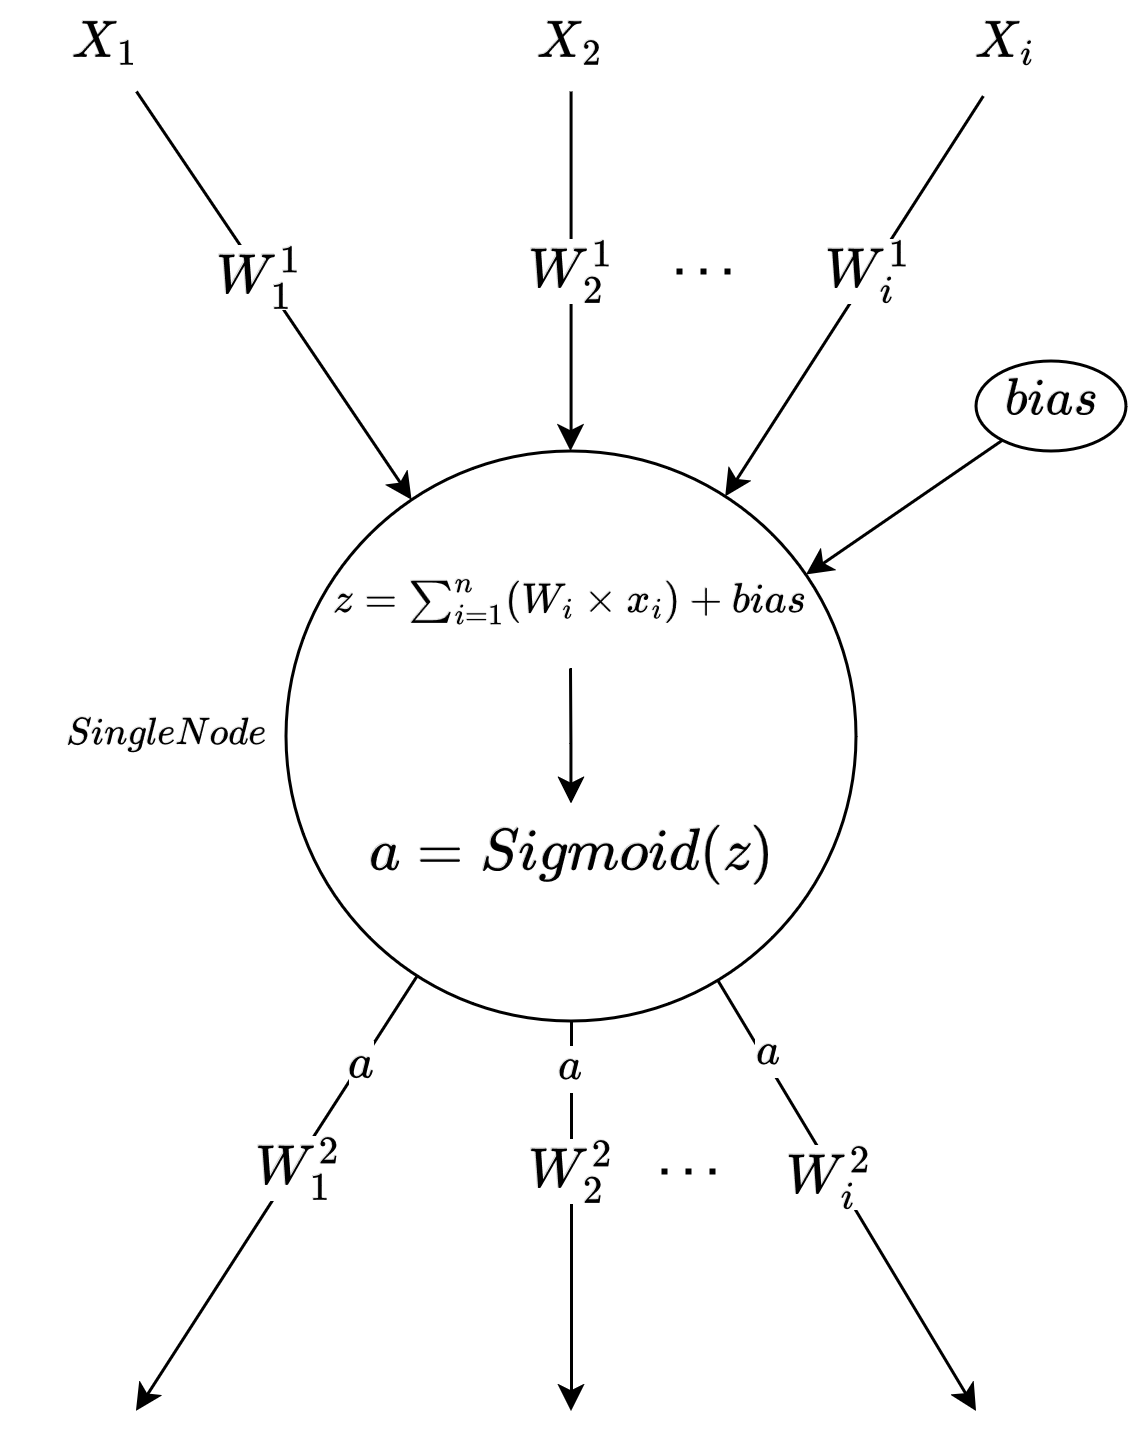
\includegraphics[width=0.5\linewidth]{template//figures/singlenode.png}
    \caption{Forward propagation zoomed in single node}
    \label{fig:singlenode}
\end{figure}


\subsection{Backpropagation}

The mathematical concept of backpropagation was first introduced as a reverse mode of automatic differentiation without direct use of neural networks (\cite{linna}). Later as a part of training the neural networks referred to as backpropagation. With forward propagation, we can produce outputs of the neural network. Backpropagation is an algorithm that is used to find the impact of each weight and bias term on the prediction error. Prediction error, also known as the loss or cost function, defines the disparity between the predicted and desired output. As the correct label is often presented as a single numerical value it needs to be converted into a similar representation as the output of the network. This can be done with one-hot encoding. A single sample from a dataset with 9 possible classes: \(\hat{y} = \{ {0.12}_1, {0.02}_2, \ldots,{0.33}_9 \}\) where the correct label is 2, can be one-hot encoded to \(y = \{ {0}_1, {1}_2, \ldots,{0}_9 \}\). There are multiple ways of calculating the difference or loss between the correct label and the predicted one. One of them is cross-entropy which is suitable for multiclass classification. 
\[\mathrm{CE}(y,\hat{y}) = -\sum_{l}^{L} y_{l} \log(\hat{y}_{l})\]

With backpropagation, we calculate the gradients of the loss function with respect to weights and bias terms. Backpropagation is sometimes misunderstood as the algorithm that optimizes the network (\cite{Goodfellow-et-al-2016}). The gradients can be thought of as a partial derivatives in a vector. We calculate these gradients for each layer moving backward from the output towards the input layer by layer. This is done because, with this approach we can use the chain rule to effectively use the already calculated values from previous layers to reduce the computation time. Backpropagation in FFNN multiclass classification with two input features, two hidden layers, and three output classes is illustrated in \ref{fig:backprop}, where \(L\) is used as the notation for the loss.

\begin{figure}
    \centering
    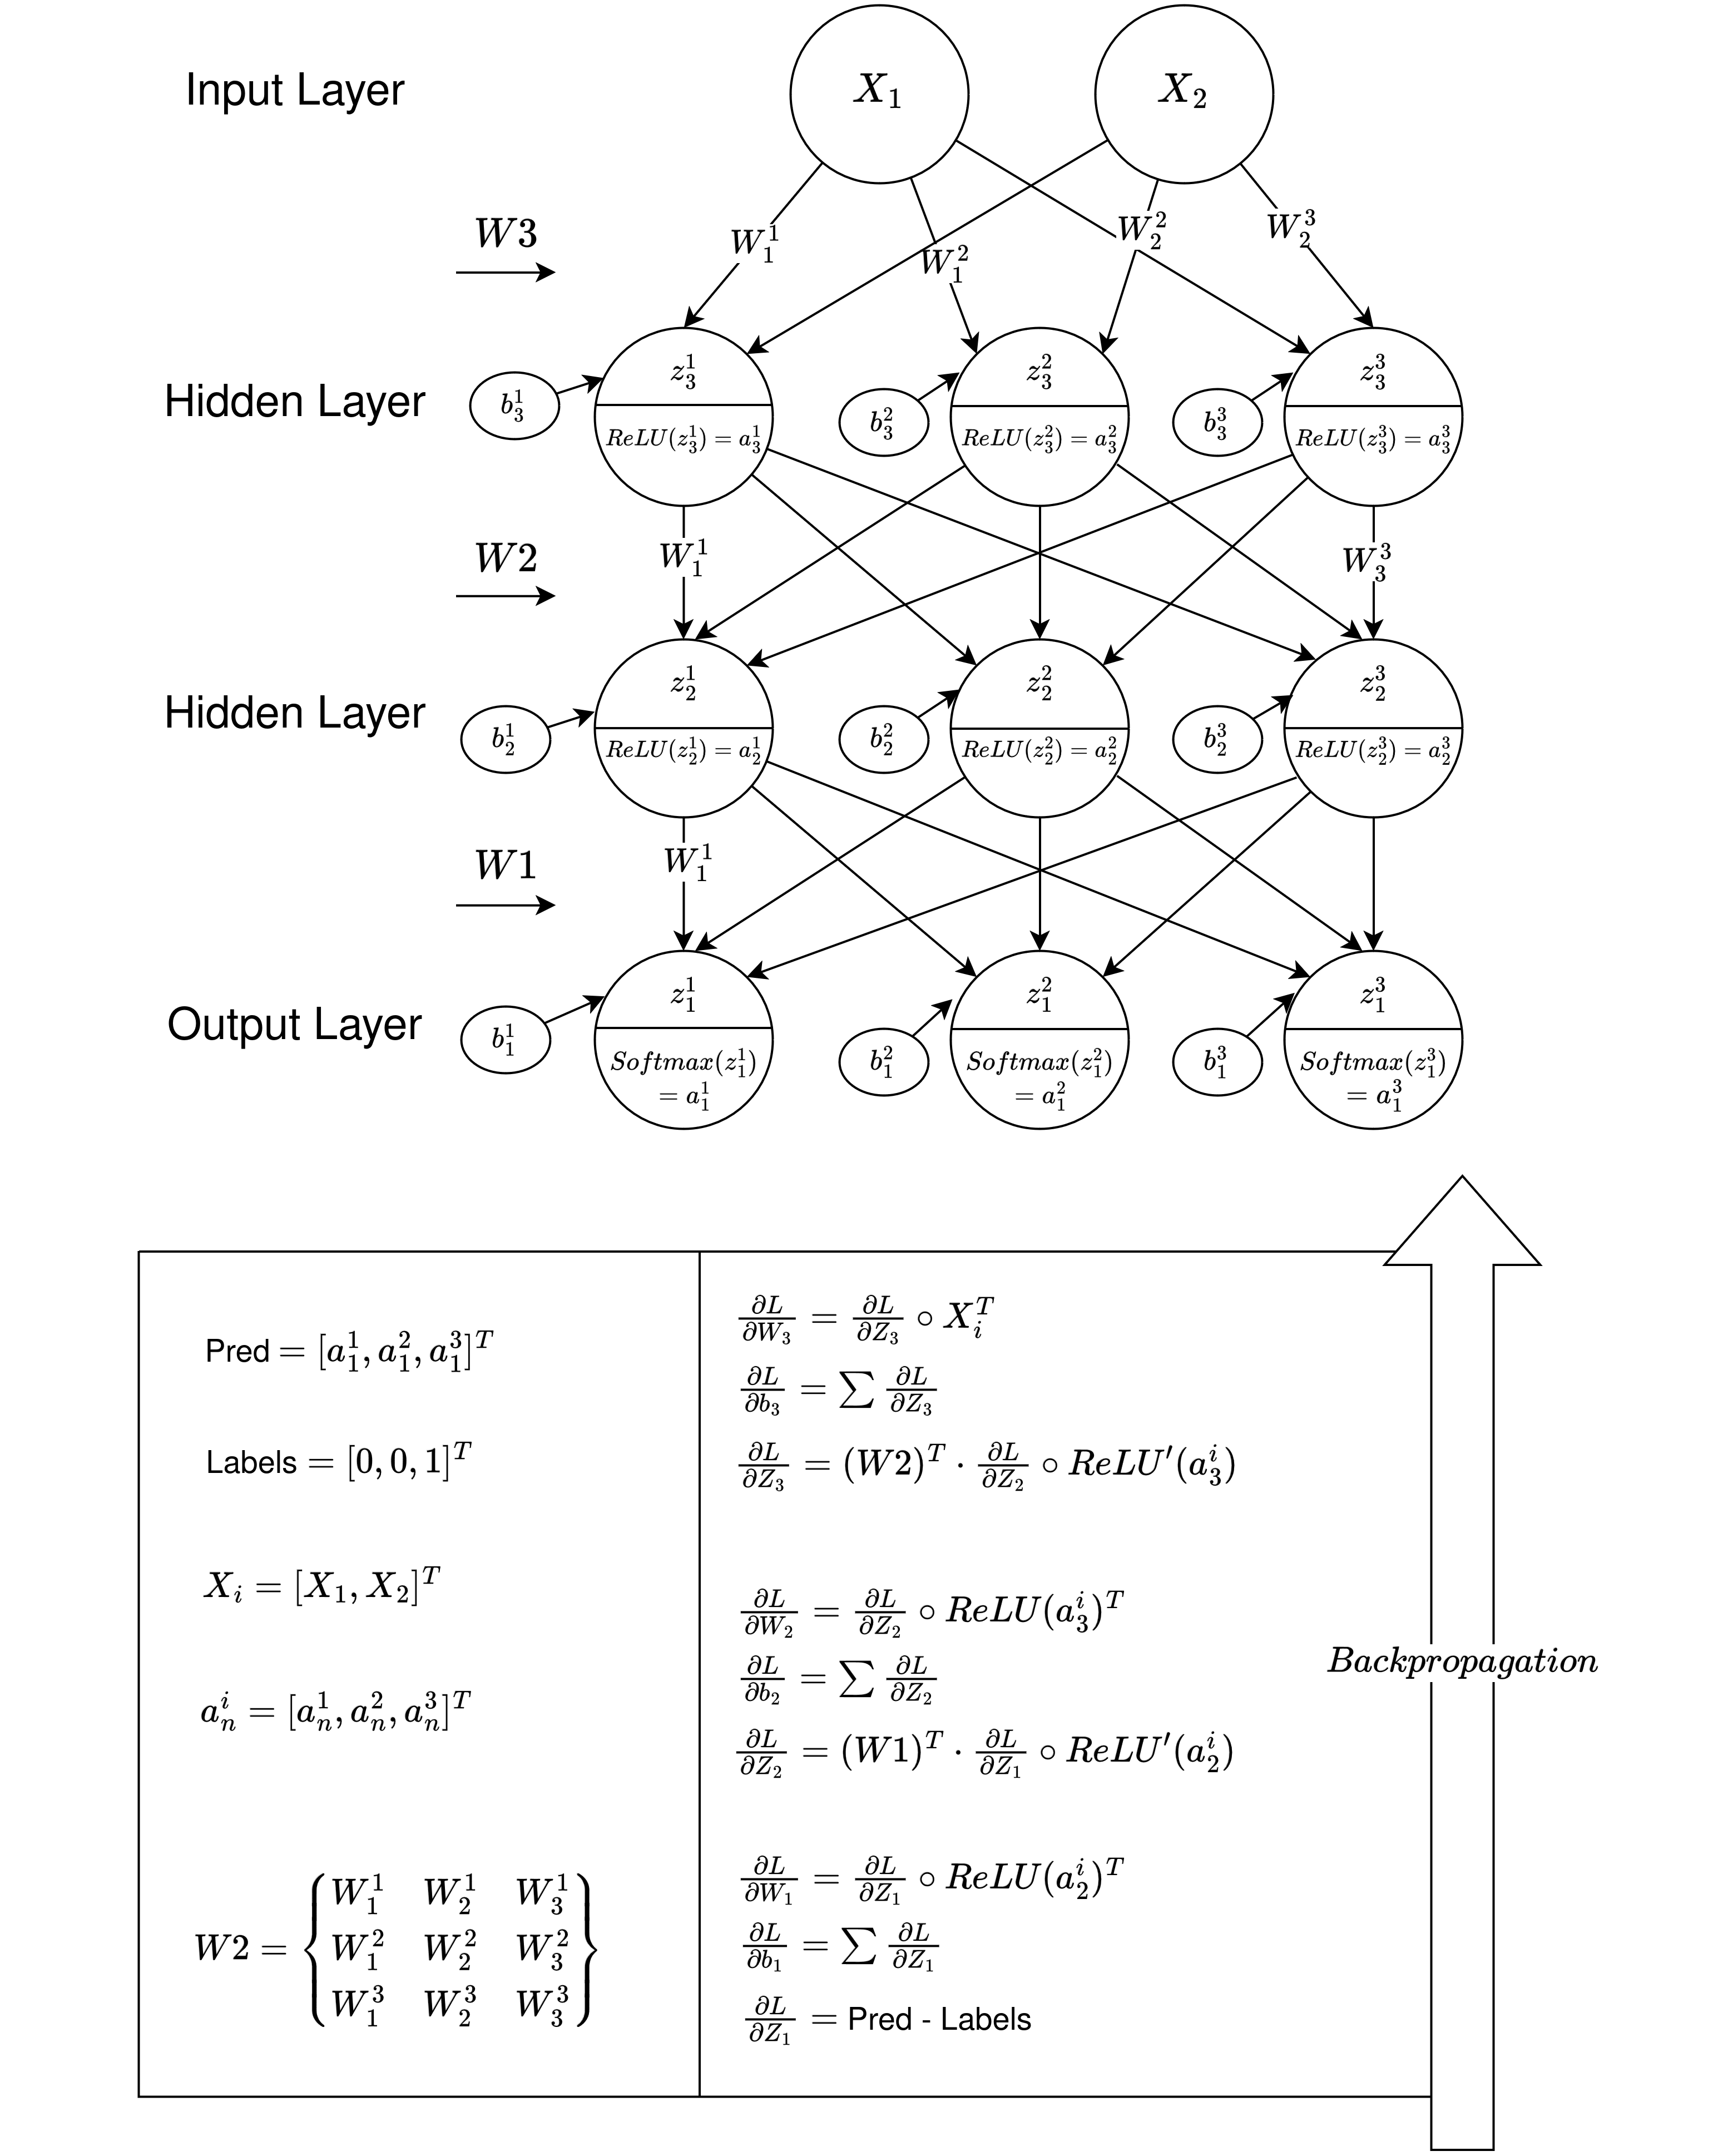
\includegraphics[width=1\linewidth]{template//figures/backpropfigVersionFinal1(1).png}
    \caption{Backpropagation}
    \label{fig:backprop}
\end{figure}

\subsection{Stochastic gradient descent}

Stochastic gradient descent (SGD) is an algorithm to optimize the neural network to minimal loss using forward and backpropagation. Some researchers have suggested that SGD may be the most commonly used algorithm to optimize neural networks (\cite{NIPS2012_6aca9700}). Weights and biases are essentially the values that we want to optimize, so the network output loss is minimized. Most of the deep learning algorithms are based on SGD (\cite{Goodfellow-et-al-2016}), so it can be seen as a fundamental part of deep learning.

The optimization for weight and biases with SGD happens after every sample. A sample is forward propagated through the network to produce predictions. Then the predictions are used to calculate loss and backpropagation is used to find the gradients to weights and biases. These gradients are then used to tune the weights (\(W_{i}\)) and biases: (\(b_{i}\))
\[W_{i} = W_{i} - \alpha \frac{\partial L}{\partial W_{i}}\]
\[b_{i} = b_{i} - \alpha \frac{\partial L}{\partial b_{i}}\]
Here \(\alpha\) is some scalar that we use to define the step size towards the direction defined by the negative gradient. The gradient points in the fastest increasing direction, so by using a negative gradient, these parameters can be adjusted toward the direction that decreases the loss function. By repeating the steps defined above for multiple samples multiple times, we can find the local minima for the loss. By optimizing the weights and biases to perfection, we train the network to produce minimal error with the training data. This leads to a problem called overfitting. Overfitting happens when we get flawless outputs with the training data but can't generalize to unseen data (\cite{overfit}). The goal of the training is to optimize the network to produce correct labels with unlabeled data, so by overfitting, we fail to achieve this goal.

Training data is commonly split into testing and training data (\cite{Goodfellow-et-al-2016}). During the training and splitting the data is shuffled. Test data gives us a portion of the data that we don't use during the training and can be used for testing as unseen data to the network. This helps to identify the overfitting and shows more accurately how the network performs outside the data it has learned from. Additional parameters to the network that are used in training are called hyperparameters. Learning rate or \(\alpha\) is a hyperparameter. The training loop goes through the whole training dataset multiple times during the optimization, "epoch" is a hyperparameter that defines how many times we crawl through the entire training data. Training can also be set to a halt when test data accuracy starts rising while the training data accuracy still decreases, this is considered an early stop (\cite{overfit}). Penalties to the loss function can be set to motivate lesser weights to be used. Other techniques like dropout can be added, more data can be gathered or noise added (\cite{overfit}). Dropout is a technique where random nodes are deleted during the training. Ultimately the optimal hyperparameters and techniques are case-specific but generally avoiding common known problems is helpful. 

Training may be extended, particularly with large deep networks, due to the iterative nature of SGD optimizing parameters after processing each sample. A similar algorithm is batch gradient descent, also known as batch learning. This method uses the entire training data before updating the parameters. The batch method finds the true gradient instead of an estimate as in SGD but is slower and SGD often produces better results (\cite{LECUN2000}). Mini batch gradient descent is a method where training is done via batches. Batch size is an additional hyperparameter that defines the batch size. This method splits the training data in each epoch into a mini-batch consisting of multiple samples that are then all forward propagated through the network simultaneously. Then the backpropagation is done similarly to all the predictions once, and the average gradients are used to update the weights. 


\subsection{Types of neural networks}

Based on the simple neural network many architectures have been built to suit specific domains or problems. They expand or add to the basic idea of neural networks and utilize similar algorithms in training.

Convolutional neural networks (CNN) introduce the concepts of convolution and pooling. CNNs are designed to handle data that has a grid-like topology and are therefore suitable for image-related tasks (\cite{Goodfellow-et-al-2016}). The simplified concepts of pooling and convolution for a 6x6x1 image are illustrated in Figure \ref{CnnExpl}. Values in the kernel are considered learnable weights that are tuned similarly to regular weights connecting neural networks. Multiple kernels can be used in a single convolutional layer, and these layers can be vertically stacked to capture higher dimensional features. Pooling and convolutional layers can be feature extraction layers that eventually are flattened and fed into a regular fully connected neural network that produces the output. Stride defines how much the kernel is moved when it is applied. A 3x3 kernel applied with stride = 1 to 6x6x1 would mean 16 dot products in total. If we had three-channel pictures, for example RGB, a kernel would have the same depth. Pooling layers calculate the maximum or average of the kernel-sized region that is similarly slid over the grid. Additional noise by flipping or zooming the images and padding to the borders are common methods that are applied to CNNs to reduce overfitting. CNNs can significantly reduce the number of parameters in the network compared to FFNNs (\cite{oshea2015introduction}) and capture features of the image effectively. The training follows similar steps and is based on the same fundamental algorithms as described with MLP.

\begin{figure}
    \centering
    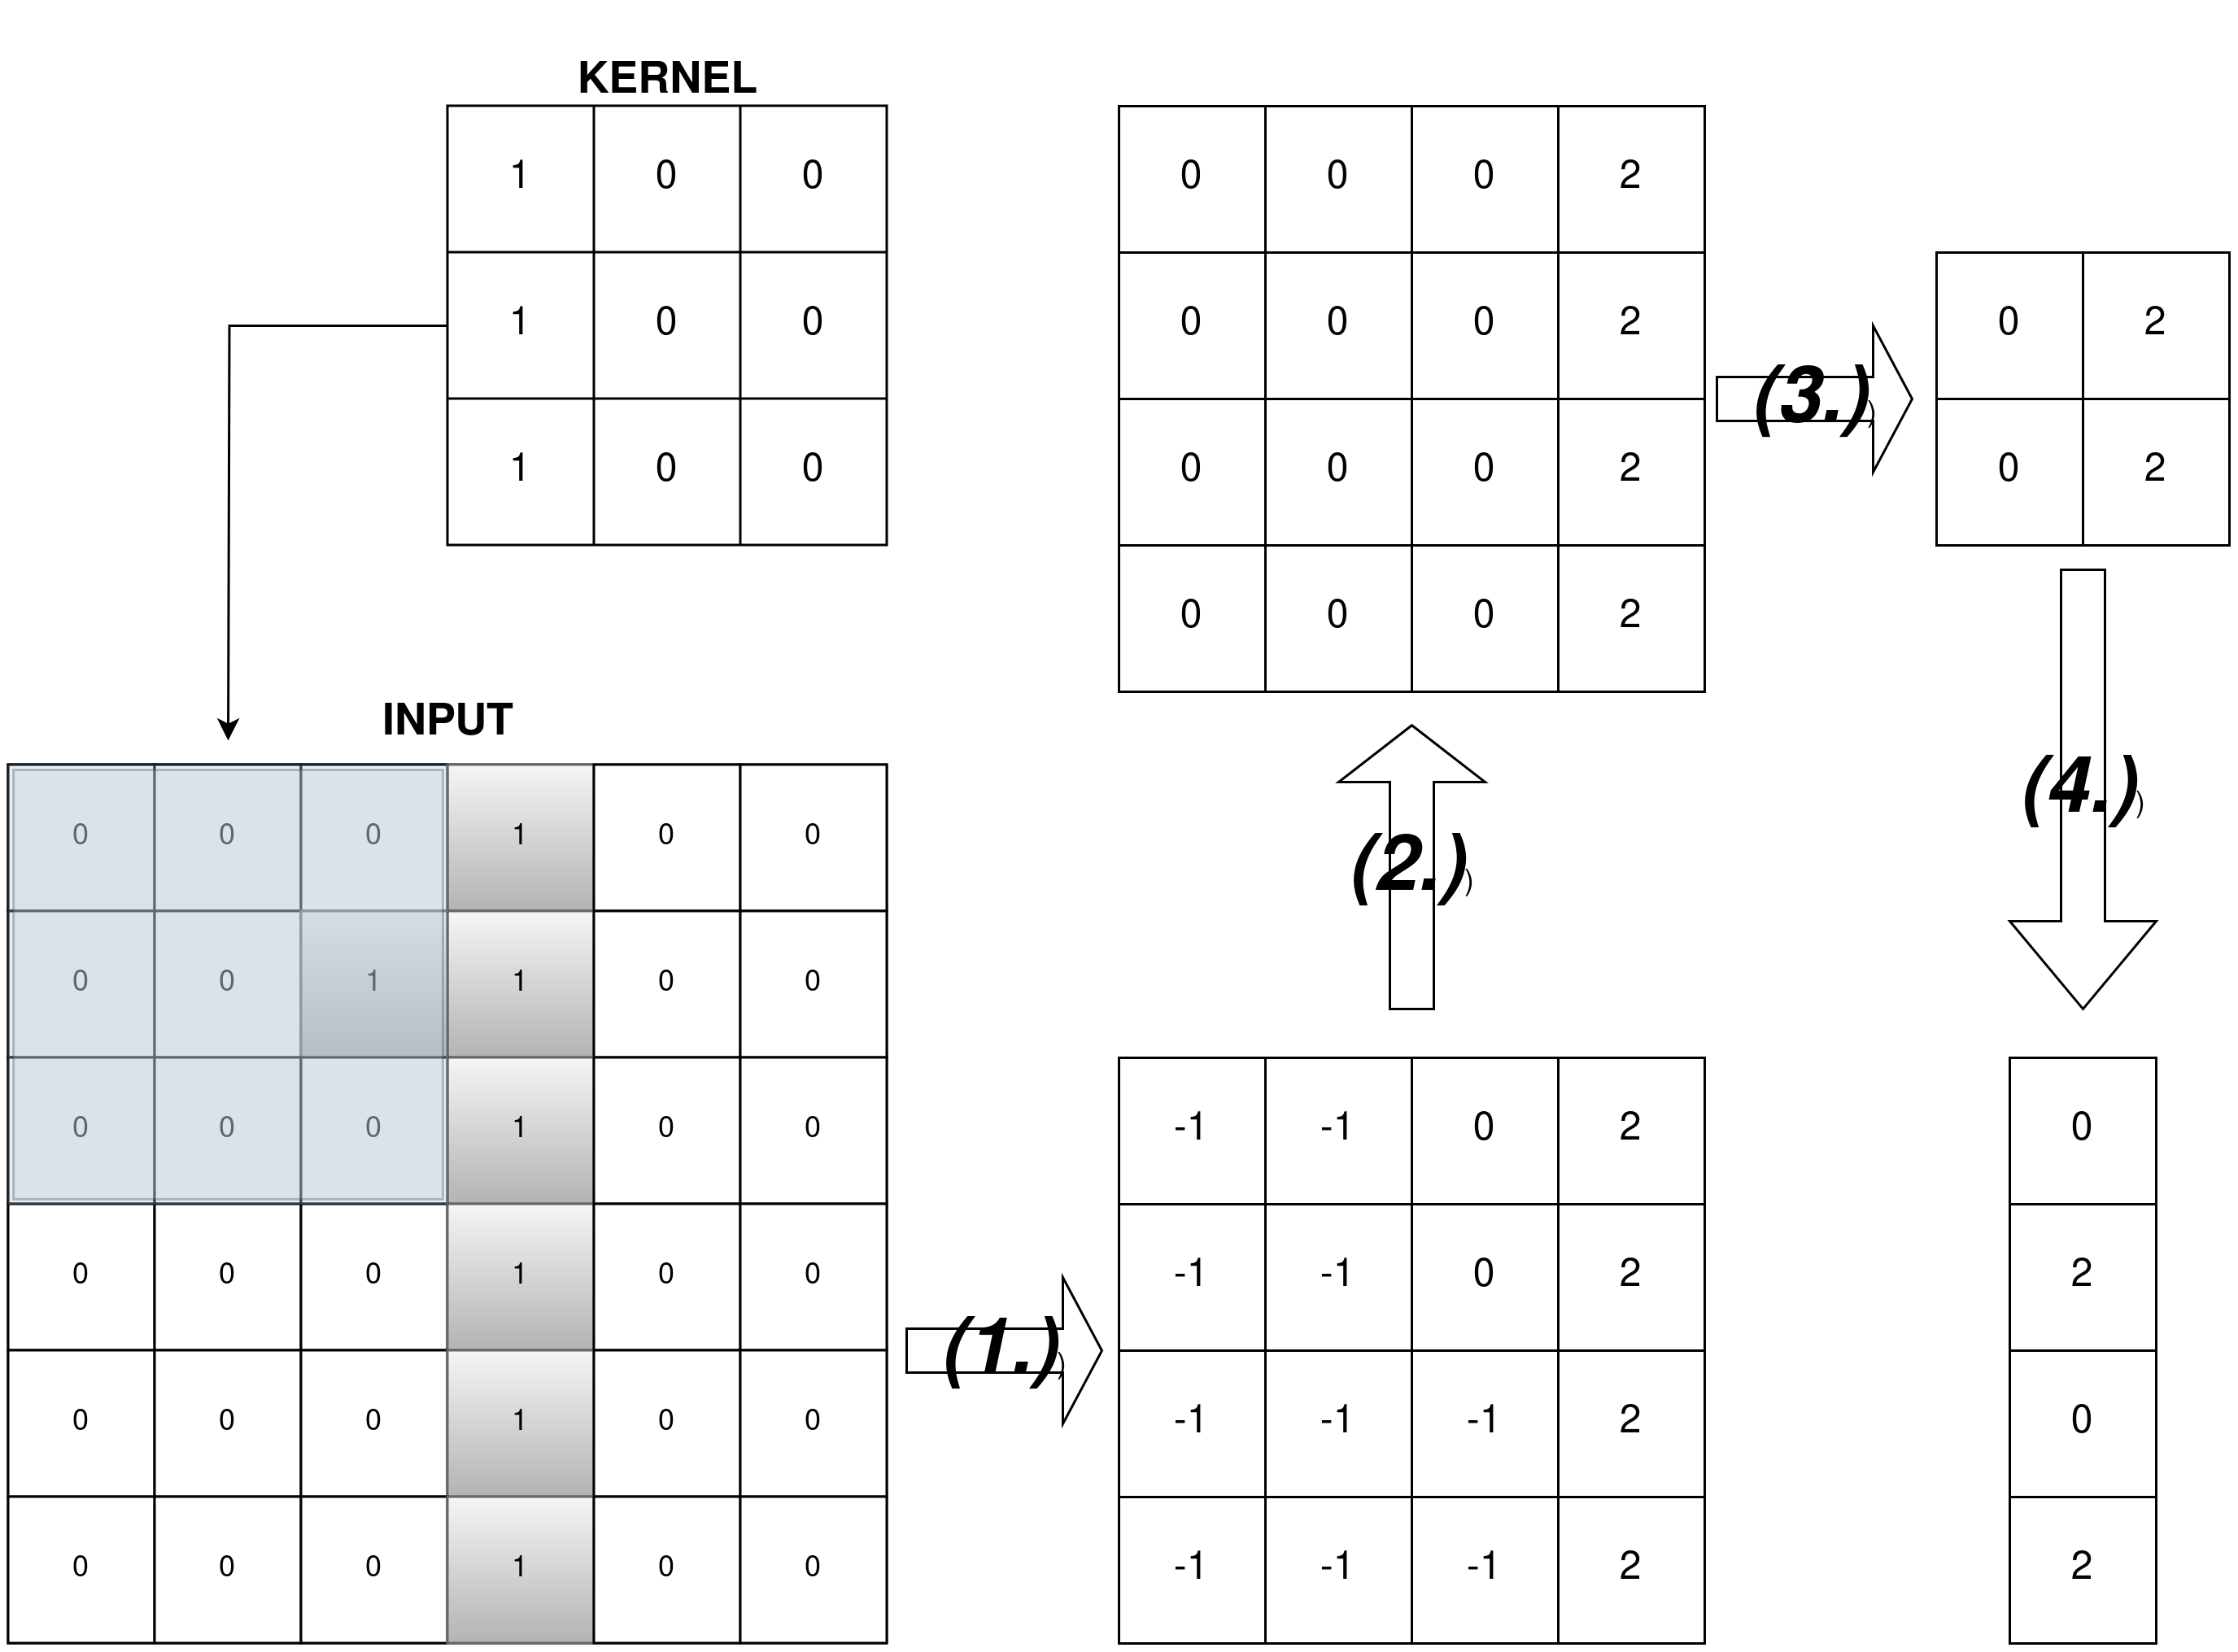
\includegraphics[width=0.75\linewidth]{CNN2EXPL.png}
    \caption{Key concepts of feature extraction layers in CNNs: (1.) Convolution with single 3x3 kernel(stride(1)) and bias[-1], (2.) Elementwise ReLU activation for the 4x4 feature map, (3.) Max-pooling (stride(2)), (4.) Flattening 2x2 to 4x1}
    \label{CnnExpl}
\end{figure}


Recurrent neural networks (RNN) are another commonly known architecture. RNNs are used with sequential data, like stock prices, weather history, or natural language. FFNNs processes all the inputs simultaneously, while RNNs processes sequential data by applying each input in order to the model (\cite{schuster1997bidirectional}). This allows the use of recurrent connections that can carry information from the previous part of the sequence to the next part. Suppose we have a sequence of some signal of integers in sequence \(X = \{ 4_{t1},5_{t2},6_{t3} \}\). The first input would be 4, and the recurrent connection \(M\) set to 0, by feedforwarding this to network, we would then have some updated \(M_1\) that could affect the next input of the sequence. The architecture shares the weight and biases so it can be easily unrolled as the only changing part is the input and the incoming value from the recurrent connection as \(M_i\). The unrolling and vanilla RNN are illustrated in \ref{RNNEXPL}. These blocks can be stacked horizontally to make the network deeper. The unrolling and the shared parameters also allow flexibility on inputs as the blocks can be unrolled according to the input sequence length. The use of activation functions, weights, and biases in the operations and connections behave similarly to the MLP. Training is done similarly with forward propagation, backpropagation, and gradient descent with some modifications to address the recurrent aspects (\cite{biglecun}). Unrolling long sequence inputs shows the main problems in RNNs, vanishing gradients, and the inability to retrain information in the memory (\cite{hochreiter1998vanishing}). Vanishing or exploding gradient is a problem where, during the backpropagation the gradients either vanish or explode, making the optimization difficult.

Long short-term memory network (LSTM) is a modification of RNNs introduced to address the vanishing gradient problem and use the memory aspect more effectively (\cite{LSTMS}). Many modifications built on top of the idea of vanilla RNN:s exist but the LSTM is one of the well-known ones. The LSTMs behave similarly to vanilla RNNs, a single block is illustrated in \ref{RNNEXPL}. LSTM block has 3 gates: forget gate, input gate, and output gate (\cite{LSTMFORGET}). These gates define the amount of memory that is kept from memory and input. Activation functions such as \(Sigmoid\) which maps input to [0,1], and \(Tanh\) that maps the input to [-1,1] are used to scale these gates.  Memory is also known as long-term memory and input as short-term memory. Similarly to vanilla RNN:s, a single block takes inputs sequentially but has 2 recurrent connections coming out of each block. These recurrent connections are not tied up with weights and therefore handle the vanishing gradient problem better.

RNNs can produce multiple and single outputs, and they can also be connected to a regular feedforward network. The main advantage of these architectures is their ability to use previous parts of sequences to influence the next parts with memory. One currently trendy and powerful architecture is a Transformer, introduced by \cite{vaswani2023attention}, which outperforms RNNs in multiple tasks. The Transformer model is built on top of the concepts of RNNs, but the specifics of the new things that this model introduces, such as the attention mechanism, will not be discussed in the scope of this thesis.

\section{Dimensionality reduction methods}

Neural networks and deep learning in general are known to need large amounts of training data. Datasets containing hundreds or more features can be described as high dimensional and are found in multiple domains such as medicine (\cite{dimredbig}). Dimensionality reduction methods aim to reduce the dimensionality and redundancy by mapping the data into a lower dimensionality space. These methods can be used for preprocessing the data in multiple machine learning classification architectures that deal with high dimensional data.

Principal component analysis (PCA) is a well-known linear dimensionality reduction method. PCA finds the lower dimensional representation of the data with the maximum amount of variance explained (\cite{van2009dimensionality}). PCA starts with the normalization of the data and then computes the covariance matrix of the data to find eigenvectors and eigenvalues for each feature. The eigenvalue represents the order of the principal components descending from the largest to the smallest. Eigenvalues also indicate the amount of variance that the component can capture. Eigenvectors can then be used to project the data into the wanted amount of these components. 

Autoencoders (AE) can also be used as dimensionality reduction methods. Autoencoders are FFNNs that aim to learn the input from reduced dimensions. This is done by forcing the data into lower dimensions and reconstructing the input from there. Multiple variations of autoencoders exist, such as multilayer autoencoders (MAE), which are simply networks with more than one hidden layer. Autoencoders hold an odd number of hidden layers and can be described with an encoder and a decoder that have shared weights (\cite{van2009dimensionality}). The bottleneck is the middle layer in the network that captures the lower dimensional representation of the input. An illustration of MAE with six hidden layers, an input layer size of \(6\), and a bottleneck size of \(3\) is found in \ref{MAE}. The encoder can be thought of as the layers before the middle layer in the network that reduces the input data to the bottleneck. The bottleneck is the layer in the middle that holds fewer nodes than there are features in the data, forcing the compression of the data. The decoder is then taught as layers after the bottleneck reconstructing the input from the bottleneck. By training this kind of network we can learn a lower-dimension representation of the data by using the data from the bottleneck layer that is forced to produce it.

\begin{figure}
    \centering
    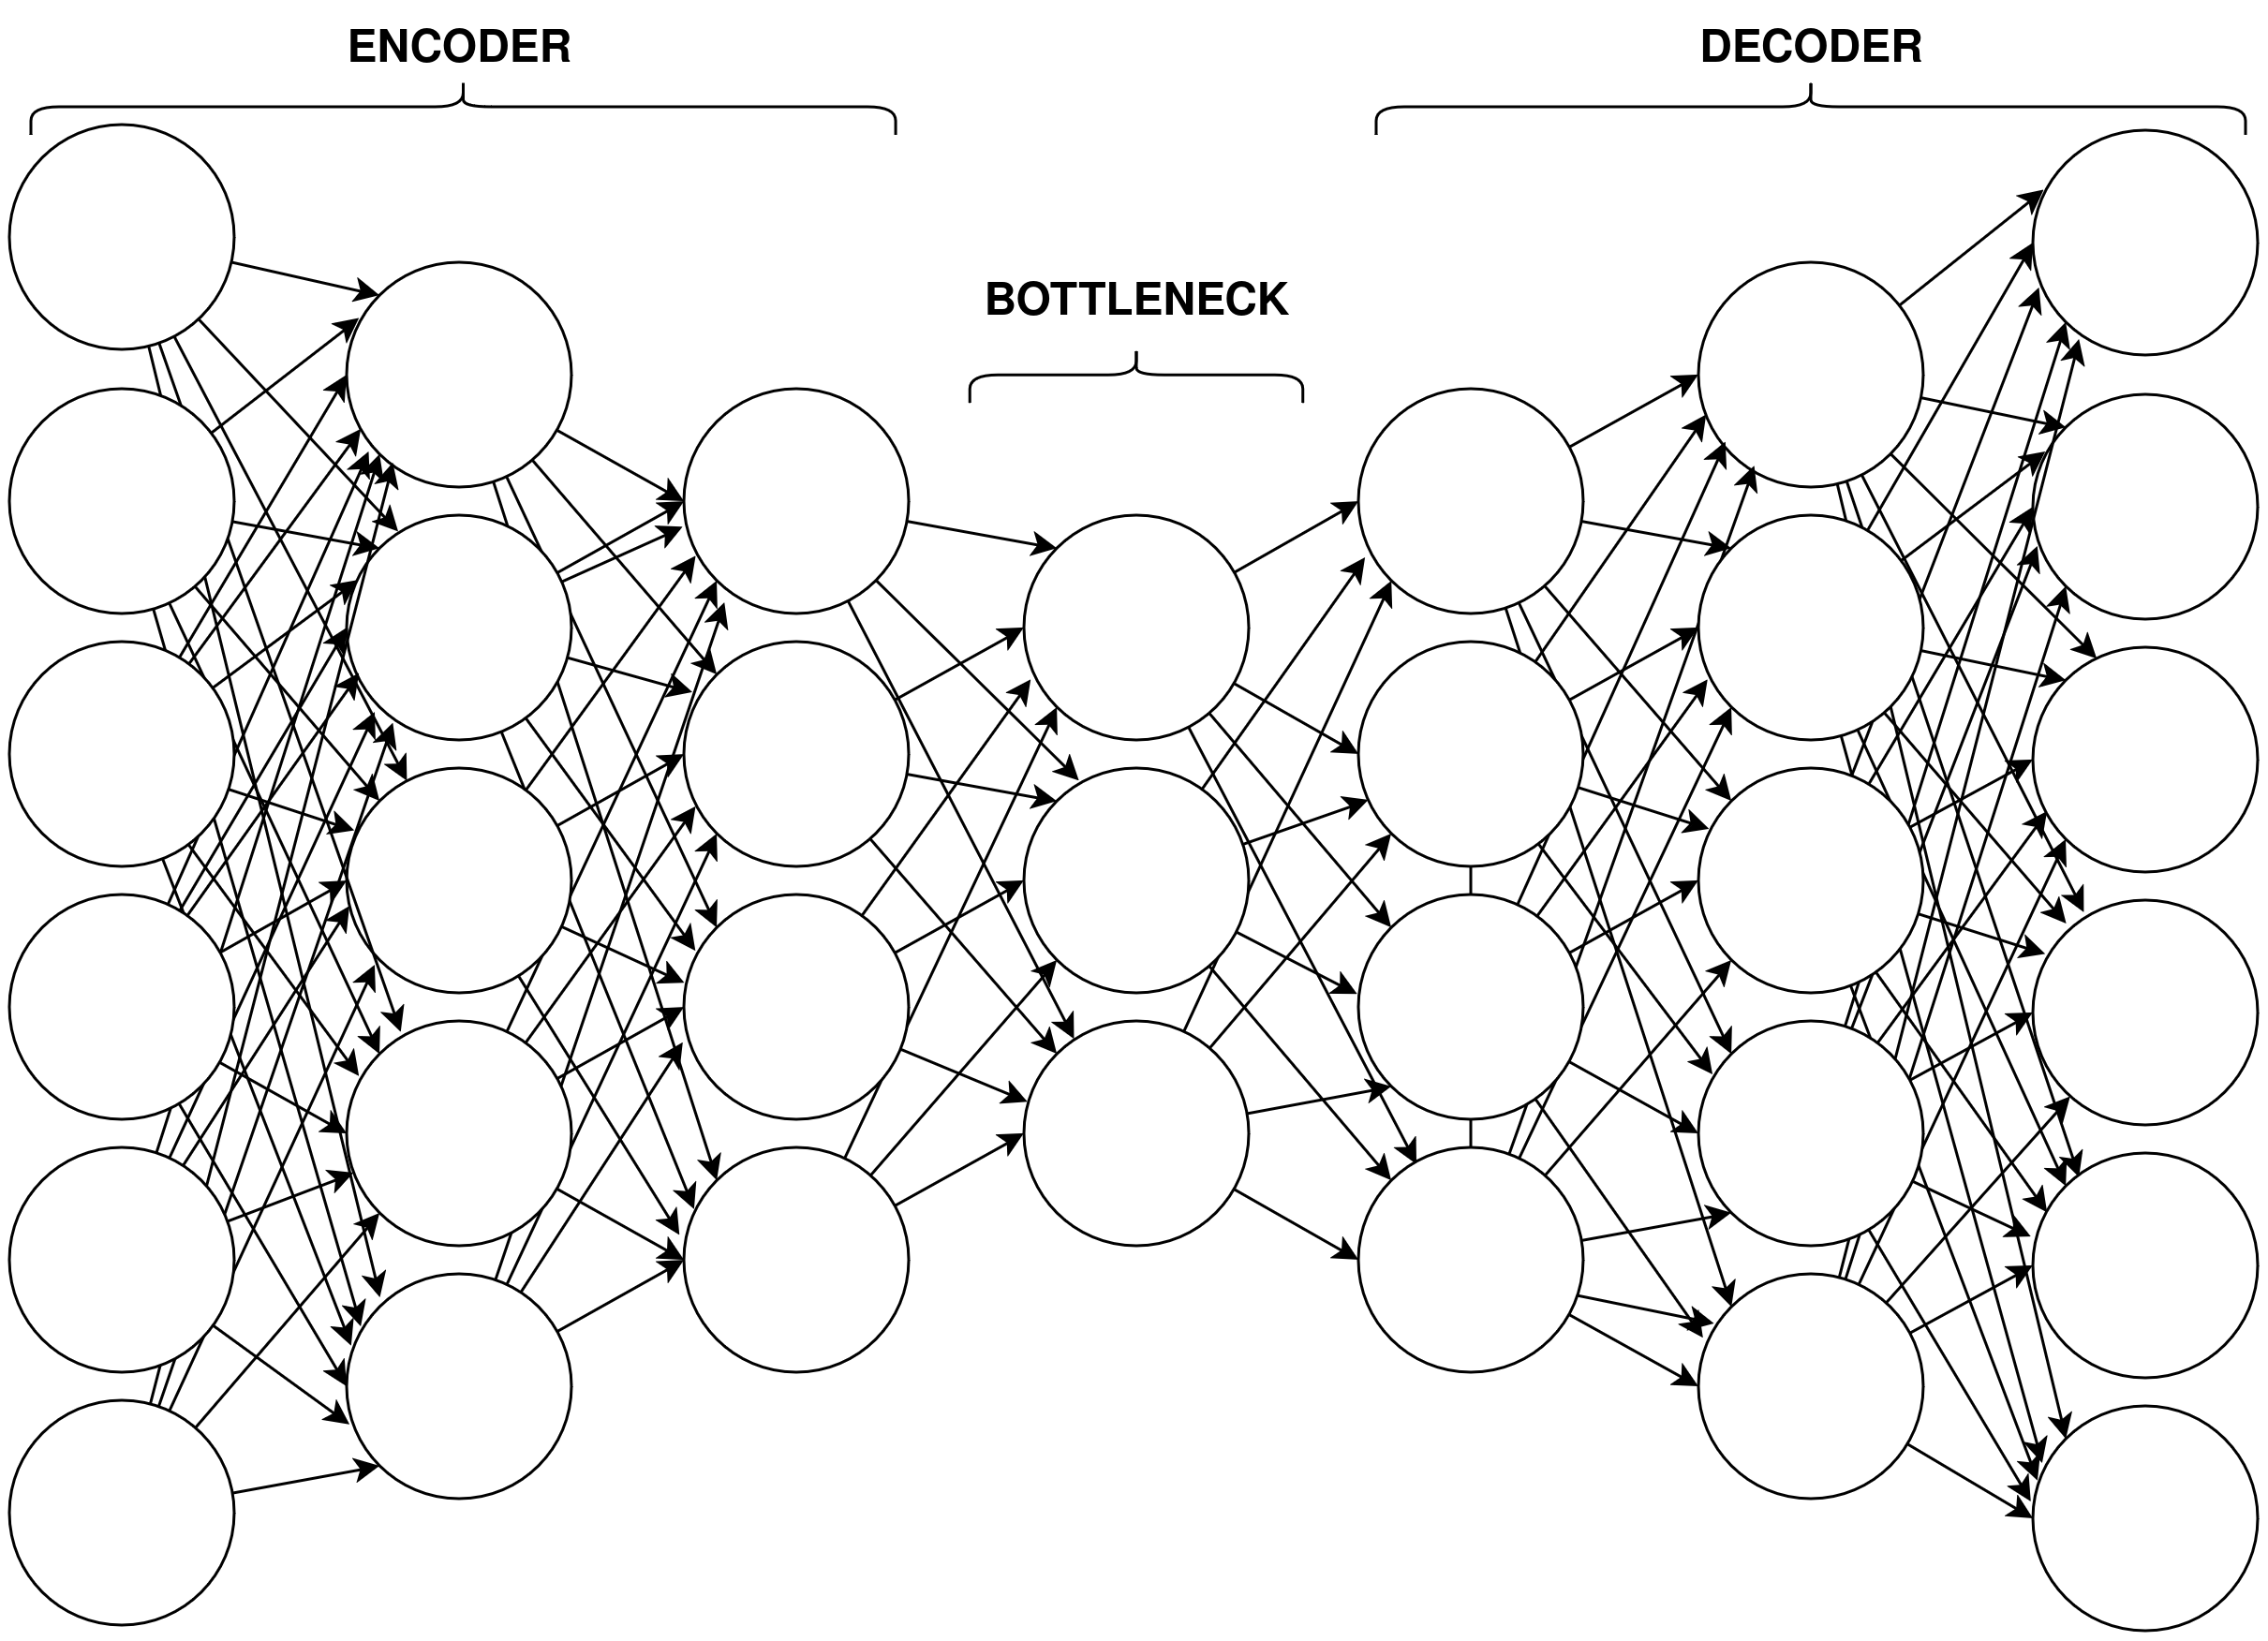
\includegraphics[width=0.75\linewidth]{template//figures/MAE.png}
    \caption{Illustration of the MAE structure}
    \label{MAE}
\end{figure}